% Options for packages loaded elsewhere
\PassOptionsToPackage{unicode}{hyperref}
\PassOptionsToPackage{hyphens}{url}
%
\documentclass[
  ignorenonframetext,
]{beamer}
\usepackage{pgfpages}
\setbeamertemplate{caption}[numbered]
\setbeamertemplate{caption label separator}{: }
\setbeamercolor{caption name}{fg=normal text.fg}
\beamertemplatenavigationsymbolsempty
% Prevent slide breaks in the middle of a paragraph
\widowpenalties 1 10000
\raggedbottom
\setbeamertemplate{part page}{
  \centering
  \begin{beamercolorbox}[sep=16pt,center]{part title}
    \usebeamerfont{part title}\insertpart\par
  \end{beamercolorbox}
}
\setbeamertemplate{section page}{
  \centering
  \begin{beamercolorbox}[sep=12pt,center]{part title}
    \usebeamerfont{section title}\insertsection\par
  \end{beamercolorbox}
}
\setbeamertemplate{subsection page}{
  \centering
  \begin{beamercolorbox}[sep=8pt,center]{part title}
    \usebeamerfont{subsection title}\insertsubsection\par
  \end{beamercolorbox}
}
\AtBeginPart{
  \frame{\partpage}
}
\AtBeginSection{
  \ifbibliography
  \else
    \frame{\sectionpage}
  \fi
}
\AtBeginSubsection{
  \frame{\subsectionpage}
}
\usepackage{lmodern}
\usepackage{amssymb,amsmath}
\usepackage{ifxetex,ifluatex}
\ifnum 0\ifxetex 1\fi\ifluatex 1\fi=0 % if pdftex
  \usepackage[T1]{fontenc}
  \usepackage[utf8]{inputenc}
  \usepackage{textcomp} % provide euro and other symbols
\else % if luatex or xetex
  \usepackage{unicode-math}
  \defaultfontfeatures{Scale=MatchLowercase}
  \defaultfontfeatures[\rmfamily]{Ligatures=TeX,Scale=1}
\fi
\usetheme[]{default}
\usefonttheme{professionalfonts}
% Use upquote if available, for straight quotes in verbatim environments
\IfFileExists{upquote.sty}{\usepackage{upquote}}{}
\IfFileExists{microtype.sty}{% use microtype if available
  \usepackage[]{microtype}
  \UseMicrotypeSet[protrusion]{basicmath} % disable protrusion for tt fonts
}{}
\makeatletter
\@ifundefined{KOMAClassName}{% if non-KOMA class
  \IfFileExists{parskip.sty}{%
    \usepackage{parskip}
  }{% else
    \setlength{\parindent}{0pt}
    \setlength{\parskip}{6pt plus 2pt minus 1pt}}
}{% if KOMA class
  \KOMAoptions{parskip=half}}
\makeatother
\usepackage{xcolor}
\IfFileExists{xurl.sty}{\usepackage{xurl}}{} % add URL line breaks if available
\IfFileExists{bookmark.sty}{\usepackage{bookmark}}{\usepackage{hyperref}}
\hypersetup{
  pdftitle={Análisis bajo asignación aleatoria},
  hidelinks,
  pdfcreator={LaTeX via pandoc}}
\urlstyle{same} % disable monospaced font for URLs
\newif\ifbibliography
\usepackage{color}
\usepackage{fancyvrb}
\newcommand{\VerbBar}{|}
\newcommand{\VERB}{\Verb[commandchars=\\\{\}]}
\DefineVerbatimEnvironment{Highlighting}{Verbatim}{commandchars=\\\{\}}
% Add ',fontsize=\small' for more characters per line
\usepackage{framed}
\definecolor{shadecolor}{RGB}{248,248,248}
\newenvironment{Shaded}{\begin{snugshade}}{\end{snugshade}}
\newcommand{\AlertTok}[1]{\textcolor[rgb]{0.94,0.16,0.16}{#1}}
\newcommand{\AnnotationTok}[1]{\textcolor[rgb]{0.56,0.35,0.01}{\textbf{\textit{#1}}}}
\newcommand{\AttributeTok}[1]{\textcolor[rgb]{0.77,0.63,0.00}{#1}}
\newcommand{\BaseNTok}[1]{\textcolor[rgb]{0.00,0.00,0.81}{#1}}
\newcommand{\BuiltInTok}[1]{#1}
\newcommand{\CharTok}[1]{\textcolor[rgb]{0.31,0.60,0.02}{#1}}
\newcommand{\CommentTok}[1]{\textcolor[rgb]{0.56,0.35,0.01}{\textit{#1}}}
\newcommand{\CommentVarTok}[1]{\textcolor[rgb]{0.56,0.35,0.01}{\textbf{\textit{#1}}}}
\newcommand{\ConstantTok}[1]{\textcolor[rgb]{0.00,0.00,0.00}{#1}}
\newcommand{\ControlFlowTok}[1]{\textcolor[rgb]{0.13,0.29,0.53}{\textbf{#1}}}
\newcommand{\DataTypeTok}[1]{\textcolor[rgb]{0.13,0.29,0.53}{#1}}
\newcommand{\DecValTok}[1]{\textcolor[rgb]{0.00,0.00,0.81}{#1}}
\newcommand{\DocumentationTok}[1]{\textcolor[rgb]{0.56,0.35,0.01}{\textbf{\textit{#1}}}}
\newcommand{\ErrorTok}[1]{\textcolor[rgb]{0.64,0.00,0.00}{\textbf{#1}}}
\newcommand{\ExtensionTok}[1]{#1}
\newcommand{\FloatTok}[1]{\textcolor[rgb]{0.00,0.00,0.81}{#1}}
\newcommand{\FunctionTok}[1]{\textcolor[rgb]{0.00,0.00,0.00}{#1}}
\newcommand{\ImportTok}[1]{#1}
\newcommand{\InformationTok}[1]{\textcolor[rgb]{0.56,0.35,0.01}{\textbf{\textit{#1}}}}
\newcommand{\KeywordTok}[1]{\textcolor[rgb]{0.13,0.29,0.53}{\textbf{#1}}}
\newcommand{\NormalTok}[1]{#1}
\newcommand{\OperatorTok}[1]{\textcolor[rgb]{0.81,0.36,0.00}{\textbf{#1}}}
\newcommand{\OtherTok}[1]{\textcolor[rgb]{0.56,0.35,0.01}{#1}}
\newcommand{\PreprocessorTok}[1]{\textcolor[rgb]{0.56,0.35,0.01}{\textit{#1}}}
\newcommand{\RegionMarkerTok}[1]{#1}
\newcommand{\SpecialCharTok}[1]{\textcolor[rgb]{0.00,0.00,0.00}{#1}}
\newcommand{\SpecialStringTok}[1]{\textcolor[rgb]{0.31,0.60,0.02}{#1}}
\newcommand{\StringTok}[1]{\textcolor[rgb]{0.31,0.60,0.02}{#1}}
\newcommand{\VariableTok}[1]{\textcolor[rgb]{0.00,0.00,0.00}{#1}}
\newcommand{\VerbatimStringTok}[1]{\textcolor[rgb]{0.31,0.60,0.02}{#1}}
\newcommand{\WarningTok}[1]{\textcolor[rgb]{0.56,0.35,0.01}{\textbf{\textit{#1}}}}
\usepackage{longtable,booktabs}
\usepackage{caption}
% Make caption package work with longtable
\makeatletter
\def\fnum@table{\tablename~\thetable}
\makeatother
\usepackage{graphicx}
\makeatletter
\def\maxwidth{\ifdim\Gin@nat@width>\linewidth\linewidth\else\Gin@nat@width\fi}
\def\maxheight{\ifdim\Gin@nat@height>\textheight\textheight\else\Gin@nat@height\fi}
\makeatother
% Scale images if necessary, so that they will not overflow the page
% margins by default, and it is still possible to overwrite the defaults
% using explicit options in \includegraphics[width, height, ...]{}
\setkeys{Gin}{width=\maxwidth,height=\maxheight,keepaspectratio}
% Set default figure placement to htbp
\makeatletter
\def\fps@figure{htbp}
\makeatother
\setlength{\emergencystretch}{3em} % prevent overfull lines
\providecommand{\tightlist}{%
  \setlength{\itemsep}{0pt}\setlength{\parskip}{0pt}}
\setcounter{secnumdepth}{-\maxdimen} % remove section numbering
\usepackage{fancyhdr}
\usepackage{lastpage}
\setbeamertemplate{navigation symbols}{}
\setbeamertemplate{footline}[page number]
\pagenumbering{arabic}
% \usepackage[mathbf,mathcal]{euler}
\usepackage{multicol}


\newenvironment{cols}[1][]{}{}

\newenvironment{col}[1]{\begin{minipage}{#1}\ignorespaces}{%
\end{minipage}
\ifhmode\unskip\fi
\aftergroup\useignorespacesandallpars}

\def\useignorespacesandallpars#1\ignorespaces\fi{%
#1\fi\ignorespacesandallpars}

\makeatletter
\def\ignorespacesandallpars{%
  \@ifnextchar\par
    {\expandafter\ignorespacesandallpars\@gobble}%
    {}%
}
\makeatother

\title{Análisis bajo asignación aleatoria}
\author{Diseño e implementación de experimentos en ciencias sociales\\
\emph{Departamento de Economía (UdelaR)}}
\date{}

\begin{document}
\frame{\titlepage}

\begin{frame}{Análisis bajo asignación aleatoria simple}
\protect\hypertarget{anuxe1lisis-bajo-asignaciuxf3n-aleatoria-simple}{}
\begin{itemize}
\tightlist
\item
  \emph{Inferencia de aleatorización (p-valores exactos para hipótesis
  nulas nítidas)}
\end{itemize}

\tiny

\begin{itemize}
\tightlist
\item
  FEDAI, capítulo 3
\item
  CISSBS capítulos 5 y 6, capítulo 9 (secciones 9.3 y 9.8), capítulo 10
  (sección 10.3)
\item
  Duflo, E., Glennerster, R., \& Kremer, M. (2007). Using randomization
  in development economics research: A toolkit. Handbook of development
  economics, 4, 3895-3962. (capítulos 4 y 7)
\item
  EGAP,
  \href{https://egap.org/resource/10-things-to-know-about-hypothesis-testing/}{10
  Things to Know About Randomization Inference}
\item
  Peng Ding, Avi Feller, and Luke Miratrix (2016), ``Randomization
  Inference for Treatment Effect Variation,'' Journal of the Royal
  Statistical Society, Series B 78: 655--671
\item
  Samii, C., \& Aronow, P. M. (2012). On equivalencies between
  design-based and regression-based variance estimators for randomized
  experiments. Statistics \& Probability Letters, 82(2), 365--370.
\end{itemize}

\normalsize

\begin{itemize}
\tightlist
\item
  \emph{Regresión y ajuste por covariables}
\end{itemize}

\tiny

\begin{itemize}
\tightlist
\item
  FEDAI, secciones 4.1, 4.2, y 4.3.
\item
  Freedman, David A. 2008. ``On Regression Adjustments in Experiments
  with Several Treatments.'' \emph{Annals of Applied Statistics} 2(1):
  176--96.
\item
  Lin, Winston. 2013. ``Agnostic Notes on Regression Adjustments to
  Experimental Data: Reexamining Freedman's Critique.'' \emph{The Annals
  of Applied Statistics} 7(1): 295--318.
\item
  Wager, Stefan, Wenfei Du, Jonathan Taylor, and Robert J. Tibshirani.
  2016. ``High-Dimensional Regression Adjustments in Randomized
  Experiments.'' \emph{Proceedings of the National Academy of Sciences
  of the United States of America} 113(45): 12673--78.
\end{itemize}
\end{frame}

\hypertarget{prueba-de-permutaciuxf3n}{%
\section{Prueba de permutación}\label{prueba-de-permutaciuxf3n}}

\begin{frame}{La señora que prueba el té \small (Fisher 1935. The Design
of Experiments. Oliver and Boyd)}
\protect\hypertarget{la-seuxf1ora-que-prueba-el-tuxe9-fisher-1935.-the-design-of-experiments.-oliver-and-boyd}{}
\begin{itemize}
\item
  ¿Tiene el té un sabor diferente según si el té se vierte en la leche o
  si leche se vierte en el té? \pause
\item
  Experimento:

  \begin{itemize}
  \tightlist
  \item
    Unidades: 8 tazas idénticas
  \item
    Aleatorización: 4 tazas al azar en las que el té se sirve primero,
    otras 4 tazas primero la leche.
  \item
    Hipótesis nula: la señora no puede notar la diferencia
  \item
    Estadístico: número de tazas clasificadas correctamente \pause
  \end{itemize}
\item
  Resultado: La señora clasificó correctamente las 8 tazas. \pause
\item
  ¿Ha ocurrido por casualidad?
\end{itemize}
\end{frame}

\begin{frame}{Test de permutación}
\protect\hypertarget{test-de-permutaciuxf3n}{}
\begin{col}{0.4\textwidth}

\tiny
\begin{table}[]
\begin{tabular}{cc|c|cc}
Taza  & Conjetura & Asignación & Escenarios             &       \\ 
\hline
1 & M  & \textcolor{blue}{M}  & \textcolor{black}{T}  \hfill  \textcolor{black}{T}  \hfill  \textcolor{black}{T}  &        \\
2 & T  & \textcolor{blue}{T}  & \textcolor{blue}{T}  \hfill  \textcolor{blue}{T}  \hfill  \textcolor{black}{M}  &        \\
3 & T  & \textcolor{blue}{T}  & \textcolor{blue}{T}  \hfill  \textcolor{blue}{T}  \hfill  \textcolor{blue}{T}  &        \\
4 & M  & \textcolor{blue}{M}  & \textcolor{black}{T}  \hfill  \textcolor{blue}{M}  \hfill  \textcolor{black}{T}  &  ...      \\ 
5 & M  & \textcolor{blue}{M}  & \textcolor{blue}{M}  \hfill  \textcolor{blue}{M}  \hfill  \textcolor{blue}{M}  &        \\ 
6 & T  & \textcolor{blue}{T}  & \textcolor{black}{M}  \hfill  \textcolor{black}{M}  \hfill  \textcolor{black}{M}  &        \\ 
7 & T  & \textcolor{blue}{T}  & \textcolor{black}{M}  \hfill  \textcolor{blue}{T}  \hfill  \textcolor{black}{M}  &        \\ 
8 & M  & \textcolor{blue}{M}  & \textcolor{blue}{M}  \hfill  \textcolor{blue}{M}  \hfill  \textcolor{black}{T}  &        \\  
\hline
\# correctas &    & 8          & 4 \hfill 6 \hfill 2 &         \\ 
\hline
\end{tabular}
\end{table}

\end{col}

\begin{col}{0.3\textwidth}
~

\end{col}

\begin{col}{0.25\textwidth}

\pause

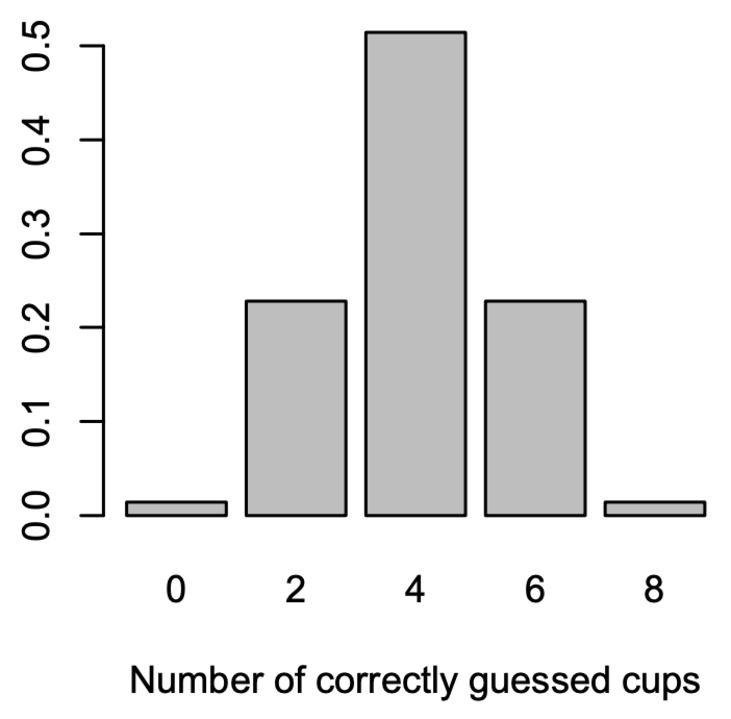
\includegraphics[width=1\textwidth,height=\textheight]{figs/dis_laidy}

\tiny

\begin{longtable}[]{@{}lrr@{}}
\toprule
term & estimate & upper\_p\_value\tabularnewline
\midrule
\endhead
Z & 1 & 0.0142857\tabularnewline
\bottomrule
\end{longtable}

\end{col}

\pause

\begin{itemize}
\item
  \(C(N, m) = \frac{N!}{m!(N-m)!} = \frac{8!}{4!4!} = 70\) \pause
\item
  Bajo la hipótesis nula, la probabilidad de que la señora clasifique
  todas las tazas correctamente es 1/70 \(=\) 0,014 \pause
\item
  Es posible que la señora posea la capacidad de diferenciar
\end{itemize}
\end{frame}

\begin{frame}{Experimentos aleatorizados (RCTs)}
\protect\hypertarget{experimentos-aleatorizados-rcts}{}
\begin{itemize}
\tightlist
\item
  ¿Por qué aleatorizar la asignación del tratamiento en los
  experimentos? \pause

  \begin{itemize}
  \tightlist
  \item
    Hace que los grupos de tratamiento y control sean ``idénticos'',
    aparte del tratamiento \pause

    \begin{itemize}
    \item
      La distribución conjunta de cualquier covariable observada (factor
      de confusión) \textbf{X} y no observado \textbf{U} previo al
      tratamiento es idéntica entre los dos grupos:
      \[P(\mathbf{X}, \mathbf{U} | T = 1) = P(\mathbf{X}, \mathbf{U} | T = 0)\],
      \pause  donde \textbf{U} incluye los resultados potenciales
      \((Y(1), Y(0)\)). \pause
    \item
      Inconfundibilidad (Unconfoundedness) de la asignación al
      tratamiento:
      \[(X, U) \perp T, \text{y en particular},  {Y(1), Y(0)} \perp T\]
      \pause
    \end{itemize}
  \end{itemize}
\item
  Nos permite cuantificar formalmente el grado de incertidumbre
\end{itemize}
\end{frame}

\begin{frame}{Inferencia por aleatorización vs a inferencia basada en
modelos}
\protect\hypertarget{inferencia-por-aleatorizaciuxf3n-vs-a-inferencia-basada-en-modelos}{}
\begin{itemize}
\tightlist
\item
  La aleatorización como
  ``\textcolor{brown}{base de razonamiento para la inferencia}''
  (Fisher)
\item
  La aleatoriedad surge del acto físico de aleatorización, que puede
  utilizarse para realizar inferencias estadísticas
\item
  También denominada
  \emph{\textcolor{brown}{inferencia basada en diseño}}
\item
  Ventaja: el diseño justifica el análisis \pause
\end{itemize}

\vspace{0.3cm}

\begin{itemize}
\tightlist
\item
  Contrasta con la inferencia basada en modelos, que asume una
  distribución de resultados potenciales
\item
  Ventaja de la inferencia basada en el modelo: flexibilidad
\end{itemize}
\end{frame}

\begin{frame}{Test de hipótesis en la inferencia causal}
\protect\hypertarget{test-de-hipuxf3tesis-en-la-inferencia-causal}{}
\begin{itemize}
\item
  ¿Cómo aprender de un efecto contrafactual
  (\(y_{Juan},T=1 \neq y_{Juan},T=0\))?
\item
  Una solución es la \textbf{estimación de efectos causales promedios}
  (ATE, ITT, LATE).
\item
  Esto es lo que llamamos el enfoque de Neyman.
\end{itemize}
\end{frame}

\begin{frame}{Test de hipótesis en la inferencia causal}
\protect\hypertarget{test-de-hipuxf3tesis-en-la-inferencia-causal-1}{}
\begin{itemize}
\item
  Otra solución es hacer \textbf{afirmaciones} o \textbf{conjeturas}
  sobre los efectos causales.
\item
  Podríamos decir: ``\emph{Creo que el efecto en Juan es 5}''. o
  ``\emph{Este experimento no tuvo ningún efecto en nadie}''. Y luego
  preguntamos ``\emph{¿Cuánta evidencia tiene este experimento sobre esa
  afirmación?}''
\item
  Esta evidencia se resume en un \(p-valor\).
\item
  A esto lo llamamos enfoque de Fisher.
\end{itemize}
\end{frame}

\begin{frame}{Ingredientes de una prueba de hipótesis}
\protect\hypertarget{ingredientes-de-una-prueba-de-hipuxf3tesis}{}
\begin{itemize}
\item
  Una \textbf{hipótesis} es una afirmación sobre una relación entre
  resultados potenciales.
\item
  Una \textbf{estadístico} resume la relación entre el tratamiento y los
  resultados observados.
\item
  El \textbf{diseño} nos permite vincular la hipótesis y el estadístico:
  calcular un estadístico que describa una relación entre resultados
  potenciales.
\item
  El \textbf{diseño} también nos dice cómo generar una
  \emph{distribución} de posibles estadísticos implícitos en la
  hipótesis.
\item
  Un \textbf{\(p\)-valor} describe la relación entre los estadísticos
  observadas y la distribución de posibles estadísticos hipotéticos.
\end{itemize}
\end{frame}

\hypertarget{inferencia-por-aleatorizaciuxf3n}{%
\section{Inferencia por
aleatorización}\label{inferencia-por-aleatorizaciuxf3n}}

\begin{frame}{Inferencia por aleatorización}
\protect\hypertarget{inferencia-por-aleatorizaciuxf3n-1}{}
\begin{itemize}
\tightlist
\item
  Nos permite hacer inferencias exactas, sin uso de distribuciones.
  \pause
\item
  Sin depender de supuestos de normalidad, etc. \pause
\item
  Sin depender de aproximaciones con muestras grandes. \pause
\item
  Verdaderamente no paramétrico, pero menos flexible.
\end{itemize}
\end{frame}

\begin{frame}{(Sharp null) Hipótesis nula nítida de ausencia de efecto}
\protect\hypertarget{sharp-null-hipuxf3tesis-nula-nuxedtida-de-ausencia-de-efecto}{}
\begin{itemize}
\tightlist
\item
  Hipótesis nula nítida:
\end{itemize}

\[H_0: \tau_i  = Y_i(1) - Y_i(0) = 0 \;\;\;\;  \forall i\]\pause

\begin{itemize}
\item
  Qué sucede si el tratamiento no afectara a nadie en absoluto?\pause
\item
  Implica que no hay efecto de tratamiento \textbf{medio}, pero no hay
  ATE (\emph{sharp null})\pause
\item
  Ejemplo sencillo con dos unidades: \(\tau_1 = 1\) y
  \(\tau_2 = -1\)\pause
\item
  Aquí, \(\tau = 0\) pero se viola la hipótesis nula nítida.\pause
\item
  Si la \emph{sharp null} es cierta, conocemos todos los resultados
  potenciales:
\end{itemize}

\[Y_i(1) = Y_i(0) = Y{i}\]
\end{frame}

\begin{frame}{La vida bajo la Hipótesis nula nítida}
\protect\hypertarget{la-vida-bajo-la-hipuxf3tesis-nula-nuxedtida}{}
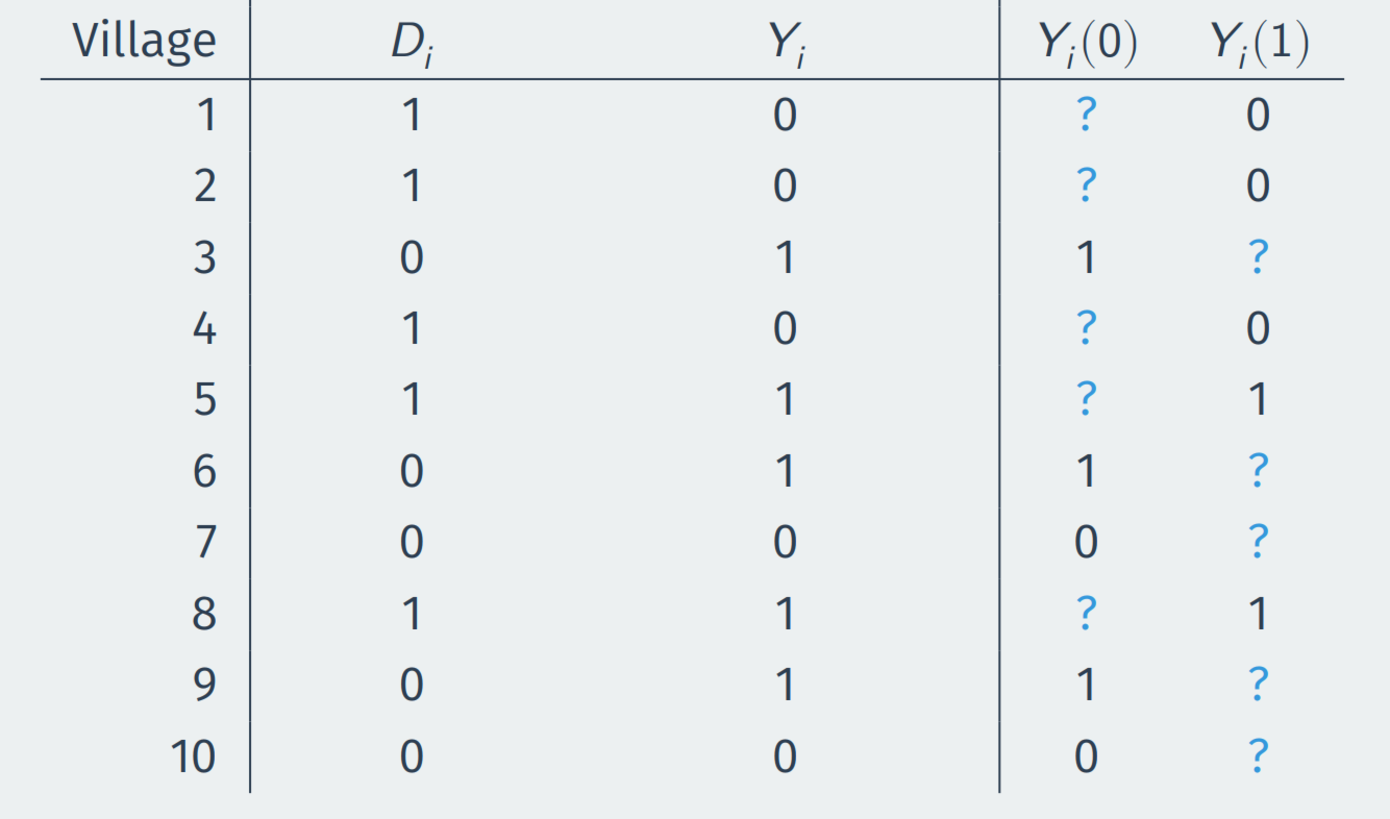
\includegraphics{figs/villages_po}
\end{frame}

\begin{frame}{La vida bajo la Hipótesis nula nítida}
\protect\hypertarget{la-vida-bajo-la-hipuxf3tesis-nula-nuxedtida-1}{}
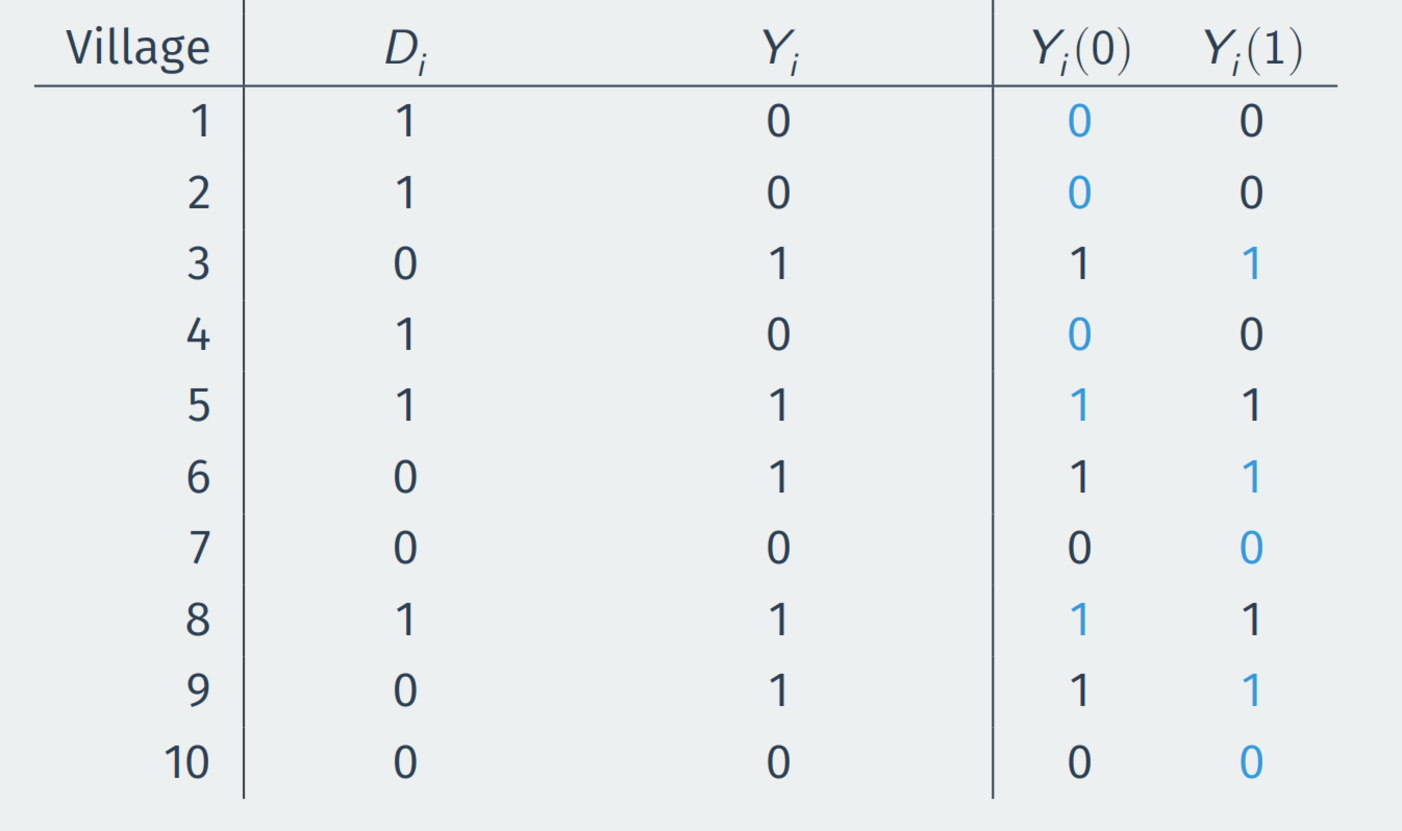
\includegraphics{figs/villages_po2}
\end{frame}

\begin{frame}{p-valor}
\protect\hypertarget{p-valor}{}
\begin{itemize}
\item
  ¿Con qué frecuencia obtendríamos un estadístico de prueba tan grande o
  más si se cumpliera la hipótesis nula nítida?
\item
  \(\tau^{obs} = \tau (\mathbf{D},\mathbf{Y},\mathbf{X})\)
\item
  \(\Omega\) es el conjunto de \(2^N\) vectores de asignación
\end{itemize}

\pause

\begin{itemize}
\tightlist
\item
  \textbf{p-valor exacto}
\end{itemize}

\[Pr(\tau \geq \tau^{obs} | Y(1), Y(0), X, H_0) = \frac{1}{\Omega_0} \sum_{\mathbf{d} \in \Omega} (\tau (\mathbf{D},\mathbf{Y},\mathbf{X}) \ge \tau^{obs})\]

\pause

\begin{itemize}
\tightlist
\item
  Frecuencia con la que \(\tau\) es mayor que el observado dividido por
  el número total de aleatorizaciones.
\end{itemize}
\end{frame}

\begin{frame}{Inferencia por aleatorización, paso a paso}
\protect\hypertarget{inferencia-por-aleatorizaciuxf3n-paso-a-paso}{}
\begin{enumerate}
\tightlist
\item
  Determinar una hipótesis nula nítida un estadístico \pause
\item
  Calcular el estadístico observado:
  \(\tau^{obs} = \tau (\mathbf{D_1},\mathbf{Y},\mathbf{X})\) \pause
\item
  Seleccionar aleatoriamente un vector de tratamiento diferente
  \(\mathbf{\tilde{D}}\) tomado de \(\mathbf{\Omega}\) \pause
\item
  Calcular
  \(\tilde{\tau}_{1}^{obs} = \tau (\mathbf{\tilde{D}_1},\mathbf{Y},\mathbf{X})\)
  \pause
\item
  Repetir pasos 3-4 para todo el espacio de aleatorización \(\Omega_0\)
  para obtener un vector
  \(\tilde{\tau} = \{\tilde{\tau}_1, \dots, \tilde{\tau}_k\}\) \pause
\item
  Calcular el p-valor:
  \(p= \frac{1}{k}\sum_{K=1}^{K}(\tilde{\tau}_K \geq \tau^{obs})\)
\end{enumerate}
\end{frame}

\begin{frame}[fragile]{Catadora de té}
\protect\hypertarget{catadora-de-tuxe9}{}
\begin{Shaded}
\begin{Highlighting}[]
\KeywordTok{plot}\NormalTok{(ri\_out, }\DataTypeTok{p =} \StringTok{"upper"}\NormalTok{)}
\end{Highlighting}
\end{Shaded}

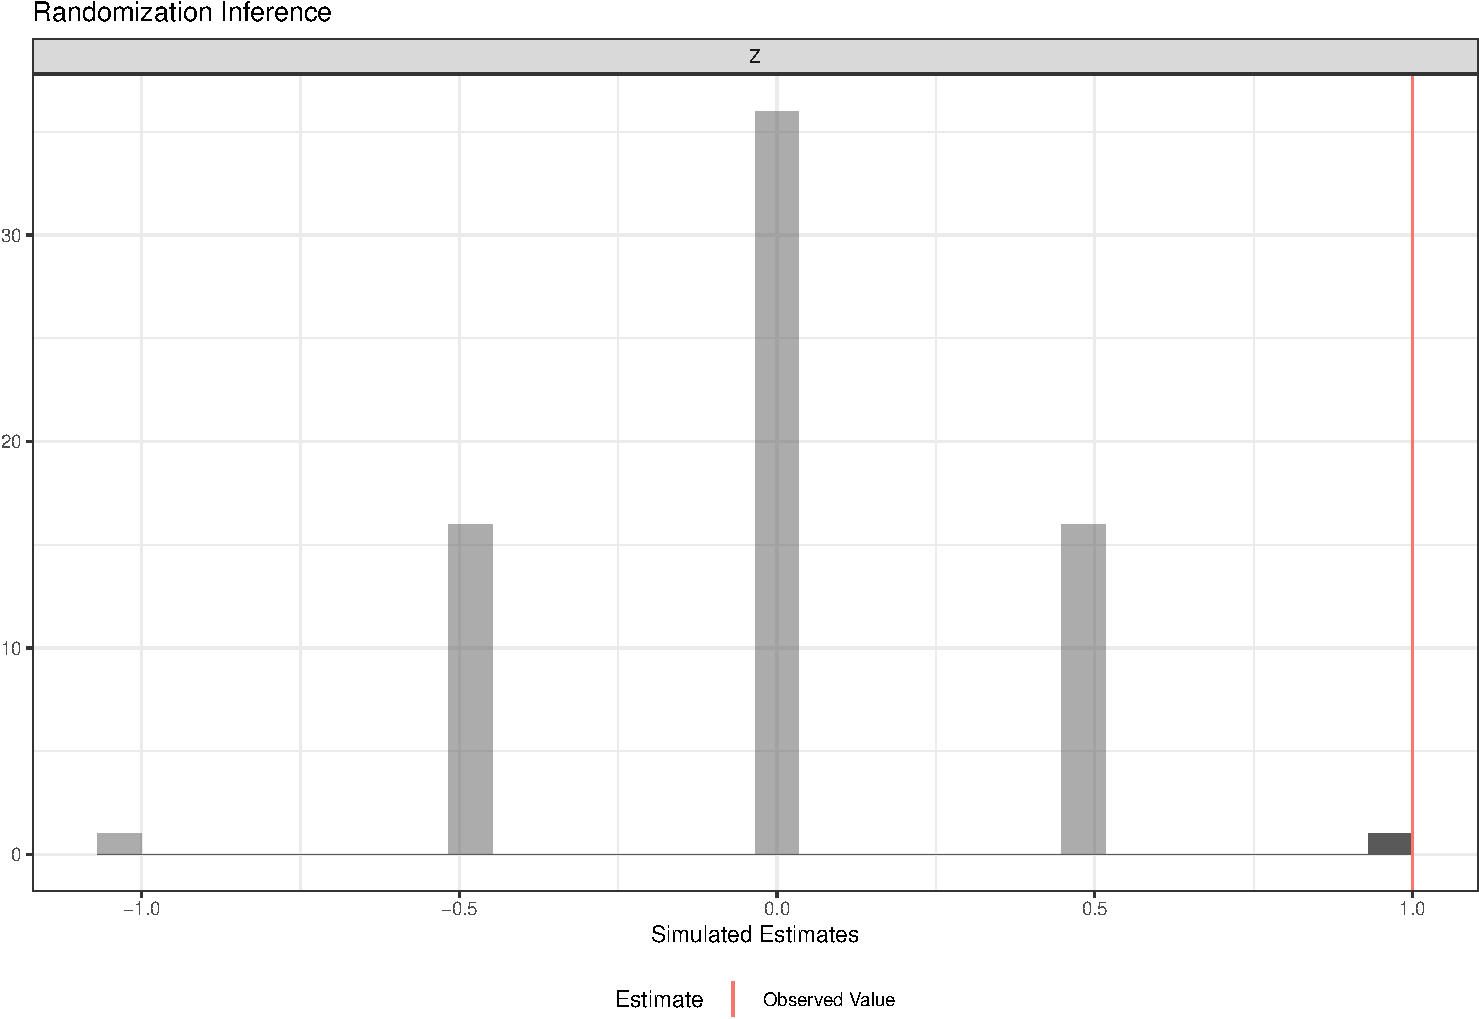
\includegraphics{Aasignacion_aleatoria_simple_files/figure-beamer/plot-1.pdf}
\end{frame}

\end{document}
